\documentclass[11pt]{article}

\usepackage[margin=1in]{geometry}
\usepackage{booktabs}
\usepackage{amsmath}
\usepackage{amssymb}
\usepackage{hyperref}
\usepackage{enumitem}
\usepackage{graphicx}

\title{Cardinal-Looking Ballots, Comparative Representations: Probing and Steering LLM Evaluator Judgments}
\author{Draft}
\date{\today}

\newcommand{\ours}{Absolute Allocation}

\begin{document}
\maketitle

\begin{abstract}
Numerical scores from LLM judges need not correspond to stable internal
magnitudes. We test this using \emph{Absolute Allocation}: a signed budget
ballot that elicits support, opposition, neutrality, and numerical intensity
alongside best-pick and weak ordinal judgments. In a 100-prompt Qwen evaluator
study, candidate-span activations linearly decode winners, pairwise ordering,
and allocation polarity. Help and hurt scores recover much of each other's
decodable information, consistent with approximately opposite readouts of a
shared comparative dimension. In contrast, linear probes consistently fail
to predict allocation magnitude after conditioning on the generated ordinal
ballot. Semantic probe directions also causally influence expressed
allocations beyond matched-norm random perturbations, although the effect is
boundary-dependent and most usable intervention outputs require deterministic
budget normalization. The central dissociation is therefore behavioral versus
representational: the elicited ballot is cardinal-looking, while the linearly
readable candidate representation is principally comparative and bipolar.
Reference display, position effects, and cross-model elicitation failures are
reported as diagnostic limits on this assay rather than separate contributions.
\end{abstract}

\section{Introduction}

LLMs are often sampled multiple times and aggregated by majority vote,
self-consistency, ranked voting, or judge selection
\cite{wang2022selfconsistency,wang2025rankedvoting,zheng2023judging}. These
methods can improve reliability when errors are independent, but LLM judges
also share correlated artifacts: verbosity preference, position effects,
format sensitivity, style preference, and plausible but wrong reasoning. A
useful voting protocol for studying LLM evaluators should therefore reveal not
only which answer is preferred, but also which answers are actively opposed,
ignored, or supported only weakly.

We study \emph{Absolute Allocation voting}. In each election, an evaluator sees
the original prompt and four candidate answers, then casts:
\begin{enumerate}[noitemsep]
    \item a single best-pick vote,
    \item a Borda-style ordinal ballot,
    \item an Absolute Allocation ballot over 100 influence cents.
\end{enumerate}
Positive cents help a candidate, negative cents hurt a candidate, and the sum
of absolute cents must be exactly 100:
\[
A=+60,\quad B=-40,\quad C=0,\quad D=0.
\]
The point is not only aggregation. The richer ballot is a behavioral assay:
best-pick gives a winner, the ordinal ballot gives relative order, and
Absolute Allocation adds signed support, opposition, neutrality, and intensity.

We distinguish four objects throughout. \emph{Ordinal information} is candidate
ordering or pairwise comparison. \emph{Polarity} is positive, zero, or negative
allocation. \emph{Intensity} is allocation magnitude conditional on the
ordinal judgment and polarity. A \emph{bipolar readout} means that help and
hurt are consistent with approximately opposite readouts of a shared decodable
dimension; it does not imply a stable cardinal utility. \emph{Cardinal
information} would require reproducible magnitude differences beyond ordinal
position. Absolute Allocation elicits all four behaviorally, but whether each
has a corresponding decodable representation is an empirical question.

This paper has four main claims.
\begin{enumerate}[noitemsep]
    \item \textbf{Linear evidence favors a bipolar comparative signal over
    residual cardinal intensity.} Candidate activations decode polarity,
    winners, and pairwise ordering, while multiple linear specifications fail
    to add out-of-sample value for magnitude after conditioning on the generated
    weak ordinal ballot.
    \item \textbf{Semantic probe directions are behaviorally causal.} Their
    activation produces allocation movement beyond matched-norm random
    strength, but this establishes influence on expressed comparative judgment,
    not direct control of a stable latent utility.
    \item \textbf{Signed ballots separate measurement from representation.}
    The ballot behavior contains polarity and magnitude beyond weak ranking;
    only part of that richer behavioral object is linearly readable at the
    tested activation site.
    \item \textbf{Context and model family delimit assay validity.} Reference
    display and presentation position change Qwen votes, while Gemma and Llama
    do not reliably produce a directly comparable signed behavioral object.
\end{enumerate}

\section{Related Work}

Self-consistency aggregates multiple sampled answers by majority vote
\cite{wang2022selfconsistency}, and recent work extends aggregation to ranked
voting rules such as Borda count and instant-runoff voting
\cite{wang2025rankedvoting}, or exploits higher-order structure beyond
majority vote \cite{ai2025higherorder}. Our ballot differs by eliciting a
bounded \emph{signed} influence budget, which makes opposition and neutrality
first-class behavioral labels rather than derived quantities. Multi-agent
debate can improve factuality but can also converge on persuasive errors
\cite{du2023debate}; our behavioral runs echo this caution, since shared
debate raised voter unanimity (53\% vs.\ 7\% under private critique) without
raising accuracy, while inference-time private critique
\cite{bai2022constitutional} preserved voter diversity. The LLM-as-a-judge
literature documents position and verbosity biases
\cite{zheng2023judging,wang2023fair}; our reference-display analysis adds
self-generated reference conditioning to that catalog of artifacts, and our position
analysis expresses primacy bias as graded support and opposition. Finally,
representation engineering asks whether high-level attributes can be read
from activations \cite{zou2023representation,zhang2023rahf} and steered by
adding activation vectors during generation \cite{turner2023activation}; we
apply both reading and steering to evaluator preference itself. Prior work
largely asks whether judge evaluations can be decoded or altered; our
contrastive question is whether signed numerical judgments correspond to
bipolar, ordinal, or cardinal internal structure.

\section{Experimental Setup}

We use 100 prompts spanning factual QA, reasoning, writing, safety, code,
business advice, instruction following, analysis, and ethics/policy. For each
prompt, \texttt{Qwen/Qwen2.5-3B-Instruct} generates four candidate answers in
different answer styles. Candidate order is shuffled during evaluation, and
style labels are hidden.

The main evaluator is \texttt{Qwen/Qwen2.5-7B-Instruct}. For behavioral
validation, we compare direct best-pick aggregation, Borda-style aggregation,
Absolute Allocation aggregation, and a single weak selector. The reported
validation specification uses 10 voters with private critique and a verified repeated
\texttt{Qwen/Qwen2.5-14B-Instruct} external judge.

We additionally run behavioral cross-model checks with
\texttt{meta-llama/Llama-3.1-8B-Instruct} and
\texttt{google/gemma-3-12b-it}. These runs reuse the same 100 prompts, the
same frozen set of 400 candidate answers, the same ballot prompt, four evaluator
repeats, and shuffled candidate presentation. They test whether the elicited
ballot behavior generalizes; they do not enter the Qwen activation probes or
steering directions reported below.

For representation analysis, each evaluator first generates its own answer to
the prompt. We then run two variants. In the \emph{visible-reference} variant,
that self-answer is shown during voting as a private reference. In the
\emph{hidden-reference} variant, the self-answer is generated but not shown
during voting; it is used only afterward as a measurement of the evaluator's
latent answer tendency. The hidden-reference design is the cleaner
mechanistic condition because it avoids direct in-context anchoring.

The primary Qwen paired experiment freezes the candidate corpus, self-answers,
candidate order, and randomized ballot-field order across conditions. A hidden
anchor uses seed 7; the visible treatment and hidden placebo both use seed 11.
The anchor yields 383 usable ballots. Because a schema bug archived display
mappings only for valid anchor ballots, 17 invalid anchor contexts are omitted
from both paired conditions; analyses are therefore complete-case and
conditioned on anchor validity. The visible and placebo runs yield 379 and 371
usable ballots, respectively.

The primary hidden representation dataset has 100 prompts, 383 usable ballots,
and four candidates per ballot, for 1{,}532 prompt-evaluator-candidate rows. We extract
candidate-span activations from the voting context and self-answer activations
from the separate self-answer context. Probes use prompt-grouped
cross-validation. The primary probe preselects layer 16 by architecture depth
and replays the exact chat-formatted ballot context; feature-family and target
comparisons remain exploratory.

The exact signed budget remains nontrivial: 338 of 383 usable hidden ballots
are natively valid. Restricting probes to these ballots leaves activation-layer
results essentially unchanged (best-pick AUC 0.750 versus 0.751 overall,
signed-top AUC 0.799 versus 0.800, help 0.693 versus 0.698, hurt 0.728 versus
0.725, and allocation $z$ score $R^2=0.217$ versus 0.219).

Table~\ref{tab:experimentmap} separates the experimental versions and their
units. We reserve \emph{exact-context replay} for identical saved inputs,
orders, and prompt construction. A \emph{natively budget-valid} output parses
and satisfies the absolute budget without rescaling; a \emph{normalized}
allocation has parseable signed values divided by their absolute total;
\emph{usable} includes either; and \emph{unusable} means no complete finite
allocation remains after retries. Thus ``exact context'' does not imply native
budget validity.

\begin{table}[h]
\centering
\small
\begin{tabular}{p{1.15in}p{0.65in}p{0.55in}p{1.05in}p{2.15in}}
\toprule
Experiment & Model & Prompts & Effective unit & Purpose \\
\midrule
Behavioral validation & Qwen & 100 & prompt & Aggregation sanity check \\
Primary probing & Qwen-7B & 100 & 383 ballots & Representation \\
Reference display & Qwen-7B & 100 & paired prompt & Context stress test \\
Cross-model elicitation & Llama/Gemma & 100 & ballot & Measurement invariance \\
Activation steering & Qwen-7B & 25 & 50 ballot clusters & Intervention \\
\bottomrule
\end{tabular}
\caption{Experiment map. Probe candidate rows and intervention generations are
repeated observations; cross-validation groups by prompt and steering standard
errors cluster by ballot.}
\label{tab:experimentmap}
\end{table}

\section{Behavioral Measurement and Diagnostic Checks}

The aggregation result is mainly a sanity check that the ballots are
behaviorally meaningful. Under the verified 14B judge, 10 voters with private
critique give the results in Table~\ref{tab:main14b}. Absolute Allocation is
competitive and has the best exact match among the direct voting methods, but
the margin over Borda-style aggregation is not decisive. We therefore treat
aggregation as validation, not the intellectual center of the paper.

\begin{table}[h]
\centering
\begin{tabular}{lccc}
\toprule
Method & $n$ & Exact match & Tie-inclusive match \\
\midrule
Direct best pick & 100 & 0.34 & 0.49 \\
Direct Borda-style & 100 & 0.35 & \textbf{0.50} \\
Direct Absolute Allocation & 100 & \textbf{0.37} & 0.47 \\
Single weak selector & 100 & 0.26 & 0.41 \\
\bottomrule
\end{tabular}
\caption{Behavioral validation under verified
\texttt{Qwen/Qwen2.5-14B-Instruct} external judge ($n=100$ prompts; 95\%
binomial intervals on these rates are roughly $\pm 10$ points).}
\label{tab:main14b}
\end{table}

\subsection{Reference-Answer Display Effects}

The Qwen reference-display comparison reuses exact self-answers, candidate order, and
ballot-field order. The same-seed visible-versus-hidden-placebo contrast changes
the elected winner on 45\% of prompts for best-pick, 38\% for Borda-style
aggregation, and 24\% for Absolute Allocation. The anchor-versus-placebo
comparison gives a seed-instability floor of 9\%, 12\%, and 10\%. Separately,
anchor-versus-visible change rates are 46\%, 39\%, and 26\%, yielding net rate
differences of 37, 27, and 16 percentage points. These differences are
descriptive, not automatically causal corrections. Paired McNemar tests
compare, prompt by prompt, the indicator that anchor-versus-visible changed the
winner with the corresponding anchor-versus-placebo indicator ($p<0.002$ for
each method; $p<10^{-9}$ for best-pick). The effect is largest for best-pick and
smallest for Absolute Allocation, consistent with richer ballots producing more
stable winners. On paired candidate rows, visible references lower mean allocation
by 0.019, change allocation polarity on 24.3\%, increase hurt from 36.8\% to
42.7\%, and reduce neutrality from 3.3\% to 0.9\%.

The Llama companion experiment isolates display more tightly. The visible run reuses
the exact saved self-answer and candidate order from the hidden run. All
400 self-answer texts match; 369 ballots parse in both conditions, spanning 99
prompts. Table~\ref{tab:anchoringpaired} reports winner changes after
aggregating only voters parsed in both conditions. Best-pick winners change on
27.3\% of prompts (95\% Wilson interval 19.5--36.8\%), while Borda and
Absolute Allocation winners change on 11.1\% and 10.1\%. Restricting to the
77 prompts with all four voters paired gives nearly identical rates: 28.6\%,
10.4\%, and 11.7\%.

\begin{table}[h]
\centering
\begin{tabular}{lccc}
\toprule
Condition & Best-pick & Borda-style & Absolute Allocation \\
\midrule
Qwen, exact inputs and same seed & 45.0\% & 38.0\% & 24.0\% \\
Qwen, seed-only placebo floor & 9.0\% & 12.0\% & 10.0\% \\
Qwen, net difference from floor (pts) & \textbf{37.0} & \textbf{27.0} & \textbf{16.0} \\
Llama, exact paired inputs ($n=99$) & 27.3\% & 11.1\% & 10.1\% \\
Llama, four paired voters ($n=77$) & 28.6\% & 10.4\% & 11.7\% \\
\bottomrule
\end{tabular}
\caption{Aggregate winner changes between hidden- and visible-reference
conditions ($n=100$ prompts). Qwen's primary contrast compares the visible run
directly with a hidden placebo at the same seed and exact paired inputs; the
net-difference row subtracts the seed-instability rate from the separate
anchor-versus-visible change rate. McNemar tests compare the two per-prompt
change indicators rather than testing the subtraction itself ($p<0.002$).
Llama lacks a same-seed placebo but reuses exact self-answers and
presentation orders and retains only ballots parsed in both conditions.}
\label{tab:anchoringpaired}
\end{table}

Reference display also changes Llama's allocation pattern, but not in the
Qwen direction. Help rises from 34.1\% to 38.4\%, neutrality falls from 22.6\%
to 19.3\%, and hurt falls slightly from 43.3\% to 42.3\%. Thus the visible
reference shifts neutrality mainly toward support rather than making Llama
more oppositional. Candidate polarity changes on 35.1\% of paired rows.
However, only 12 ballots are natively valid in both conditions; within those
48 candidate pairs, polarity changes on 6.25\% and mean absolute allocation
movement is 0.060. Exact magnitude and polarity-change claims are therefore
substantially less secure than the best-pick result.

Reference-guided judging should consequently be treated as a first-order and
model-dependent design choice. The Qwen comparison establishes a reference-
display effect across all three aggregation rules above an estimated
seed-instability floor and shows that a visible reference makes Qwen
more oppositional (hurt rising from 36.8\% to 42.7\%, neutrality falling from
3.3\% to 0.9\%). The Llama comparison lacks a same-seed placebo and shifts
instead toward support. These outcomes are compatible with anchoring,
self-preference, consistency pressure, added information, or contrast; the
design does not distinguish among them.

\subsection{Position Bias}

Presentation order has a strong graded effect. In the hidden-reference
run, the first-shown candidate receives the best-pick vote 47.5\% of the time
versus 12.5\% for the fourth. Mean Absolute Allocation drops from 0.202 for
position 1 to 0.080 for position 4. The first-shown candidate is helped
70.0\% of the time and hurt 28.5\%; the fourth is helped 52.2\% and hurt
43.6\%. Absolute Allocation is useful here
because it exposes position bias as graded support and opposition, not only as
a top-choice artifact.

\begin{figure}[h]
\centering
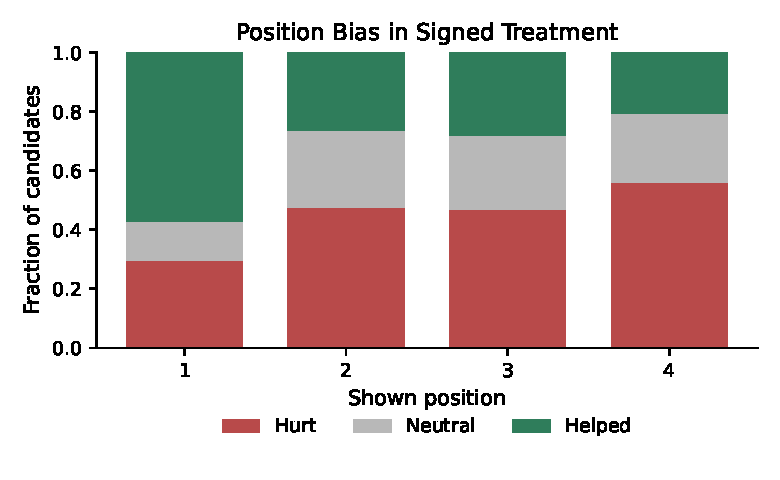
\includegraphics[width=0.68\linewidth]{paperFigs/fig_position_polarity.pdf}
\caption{Position bias in the fixed-field-order hidden-reference experiment.
The randomized-field primary experiment retains the best-pick primacy gradient but has a
more positive allocation distribution overall.}
\label{fig:positionpolarity}
\end{figure}

\subsection{Cross-Model Measurement Invariance}

The same prompt does not reliably elicit a comparable signed behavioral object from every model
(Table~\ref{tab:crossmodelballots}). Llama's parsed ballots have nearly the
same help/neutral/hurt proportions as Qwen, although Llama satisfies the
absolute-cent budget far less often and voluntarily returns a strict ranking
on every parsed ballot. Gemma has the opposite profile: it follows the output
schema and budget reliably, but usually treats Absolute Allocation as a
winner-take-all vote.

\begin{table}[h]
\centering
\small
\begin{tabular}{lrrrrrr}
\toprule
Evaluator & Parsed & Native & One-hot & Help & Neutral & Hurt \\
\midrule
Qwen2.5-7B (fixed-field experiment) & 400 & 60.5\% & 9.5\% & 33.1\% & 21.9\% & 44.9\% \\
Llama3.1-8B & 387 & 14.0\% & 7.8\% & 34.0\% & 22.5\% & 43.5\% \\
Gemma3-12B & 400 & 97.3\% & 81.8\% & 34.0\% & 64.7\% & 1.3\% \\
\bottomrule
\end{tabular}
\caption{Archived cross-model hidden-reference behavior on the same 100 prompts,
candidate answers, and fixed-field ballot prompt. Native is the fraction of 400 attempted ballots requiring
no repair or normalization; one-hot is among parsed ballots; polarity rates are among parsed
candidate rows.}
\label{tab:crossmodelballots}
\end{table}

Gemma selects candidate A on 322 of 400 ballots and gives all 100 cents to one
candidate on 327 ballots. Of 389 natively valid ballots, only six candidate rows
(0.39\%) receive negative allocation. Even when Gemma uses tied ordinal
groups, Absolute Allocation adds little information: among 201 tied candidate
pairs, only 10 receive different allocations and only two differ in sign.
This leaves no defensible native hurt class from which to estimate a bipolar
probe or intervention direction. We therefore retain Gemma as evidence that
the assay lacks measurement invariance under the current prompt, not as
evidence of a different internal preference geometry, and exclude it from
representation and steering analyses.

This collapse cannot yet be attributed wholly to Gemma's internal preference
geometry. The formatting example in the shared ballot prompt uses the real
candidate IDs, demonstrates A as best, ranks $A>B>C>D$, and assigns A all 100
cents. Candidate order is shuffled, but candidate identity is not relabeled;
Gemma's A preference persists at every shown position. Gemma may therefore be
especially susceptible to the schema example. A neutral-example or
candidate-label permutation ablation is required before interpreting its
winner-take-all behavior as intrinsic.

\section{Representation Results}
\label{sec:representation}

\subsection{Candidate Activations Predict Ballots}

Candidate activations predict the evaluator's own voting behavior in the
hidden-reference run (Table~\ref{tab:hiddenfamilies}). Candidate activations
alone carry most of the signal; self-answer-relative features add small
increments, and simple self-answer geometry alone is weak. Thus the
self-answer design is useful as an ablation, but the self-answer is not the
main source of predictive power in these linear probes.

\begin{table}[h]
\centering
\begin{tabular}{lccc}
\toprule
Target & Candidate activation & + self-answer delta & Self geometry only \\
\midrule
Voter best-pick vote & AUC 0.772 & \textbf{AUC 0.774} & AUC 0.530 \\
Voter allocation top choice & AUC 0.821 & \textbf{AUC 0.829} & AUC 0.650 \\
Voter allocation, z-scored & $R^2=0.229$ & \textbf{$R^2=0.241$} & $R^2=0.036$ \\
\bottomrule
\end{tabular}
\caption{Primary randomized-context hidden-reference feature-family comparison at the
preselected layer 16. The self-answer is generated before voting but not shown.}
\label{tab:hiddenfamilies}
\end{table}

Several secondary checks support the same conclusion. Pairwise
candidate-difference activations predict which candidate receives more
Absolute Allocation with AUC 0.787. Position is predictive by itself
(position-only best-pick AUC 0.683), but decodability survives matching on
shown position: pooled within-position AUC is 0.659 for help, 0.719 for hurt,
0.666 for best-pick, and 0.771 for allocation top choice. Randomized ballot
field order alone is at chance, and self-answer geometry gives only
$R^2=0.036$ for allocation $z$ score.

\subsection{Absolute Allocation Refines Weak Ordinal Groups}

In the fixed-field experiment, the ordinal ballot is Borda-style, but it is not canonical
strict Borda. The prompt allowed ranked groups, so the observed ordinal object
is a weak ranking with ties. This matters: only 17.5\% of hidden-reference
ballots are strict 1-1-1-1 rankings. The most common weak-ranking patterns are
[1,3] at 36.75\% and [1,2,1] at 36.75\%.

Absolute Allocation adds signed structure inside these coarse ordinal groups.
Within tied-rank candidate pairs, 47.0\% receive different allocations and
35.9\% receive allocations of different sign. Table~\ref{tab:rankpolarity}
shows dense-rank polarity. Dense rank 2 has high hurt frequency, but because
rank 2 often denotes a tied non-top group rather than strict second place, this
should not be read as evidence for systematic ``competitive opposition'' to
strict second-place candidates. In the strict-ranking subset, hurt rates
increase monotonically with worse rank: 32.86\% at rank 2, 50.00\% at rank 3,
and 61.43\% at rank 4. The safer interpretation is that Absolute Allocation
refines weak/coarse ordinal judgments.

\begin{table}[h]
\centering
\begin{tabular}{lccccc}
\toprule
Dense rank & $n$ & Help rate & Neutral rate & Hurt rate & Mean allocation \\
\midrule
1 & 400 & 0.980 & 0.020 & 0.000 & 0.584 \\
2 & 841 & 0.137 & 0.244 & 0.620 & -0.061 \\
3 & 289 & 0.066 & 0.398 & 0.536 & -0.088 \\
4 & 70 & 0.057 & 0.329 & 0.614 & -0.086 \\
\bottomrule
\end{tabular}
\caption{Dense rank from the Borda-style weak ordinal ballot versus Absolute
Allocation polarity in the fixed-field hidden-reference experiment. Dense ranks are not
equivalent to positions in a forced strict Borda ranking.}
\label{tab:rankpolarity}
\end{table}

\begin{figure}[h]
\centering
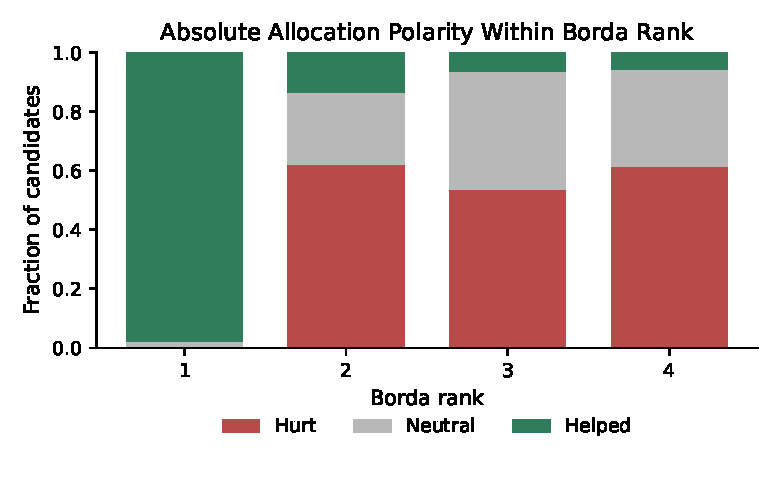
\includegraphics[width=0.68\linewidth]{paperFigs/fig_borda_rank_polarity.pdf}
\caption{Absolute Allocation decomposes each dense weak-ordinal rank into
helped, neutral, and hurt candidates. Dense rank 2 includes many tied non-top
groups, so its high hurt rate reflects signed structure inside coarse ordinal
groups, not opposition to strict second-place competitors.}
\label{fig:bordarankpolarity}
\end{figure}

Rank-matched probes show that some of this signed structure is visible in
activations. Within dense weak-ordinal rank 2, candidate activations predict
help (AUC 0.607), hurt (AUC 0.635), and neutrality (AUC 0.584), outperforming
position-only baselines (0.516, 0.523, and 0.550). The effects are modest, but
they show that the signed labels are not purely formatting noise.

\subsection{Bipolar Comparative Readout Without Residual Linear Intensity}

The key negative result is residual intensity. Borda-style weak-ordinal
targets are already predictable: in the hidden run, Borda-style $z$ score
reaches $R^2=0.148$, compared with Absolute Allocation $z$ score
$R^2=0.242$. But after regressing Absolute Allocation targets on the voter's
own ordinal-ballot features, candidate activations do not predict the
residuals. Across five prompt-grouped folds, residual mean $R^2\pm$ SD is
$-0.036\pm0.039$ for raw allocation, $-0.002\pm0.017$ for centered allocation,
$0.003\pm0.017$ for allocation $z$ score, $-0.040\pm0.027$ for positive mass,
and $-0.006\pm0.034$ for negative mass. Adding shown-position covariates does
not improve the result.

This null is not trivial: the weak ordinal ballot leaves real behavioral
variance, because most ballots contain ties and tied candidates often receive
different signed allocations. The residual result says that this extra
cardinal-looking variance yields no out-of-sample predictive value for the
linear probes, layer, token pooling, and sample tested here. This is a
consistent predictive failure across several intensity targets, not an
equivalence test. Nonlinear, distributed, later-layer, or relational encodings
remain possible, as does attenuation from noisy allocation labels or
conditioning on the generated ranking.

Support and opposition, by contrast, behave as opposite ends of one decodable
axis. Raw help/hurt direction cosines (about $-0.91$) are attenuated by low
split-half coefficient reliability (0.04 at the probe's default regularization,
rising to 0.08--0.11 at $C=0.01$). At $C=0.01$ the attenuation-corrected cosine
is nonetheless a stable $-1.00$ (50 of 50 valid split-half corrections in both
standardized and raw coordinates), destabilizing only at higher regularization,
so the cosine is only reliability-limited corroboration. Score sufficiency is
the primary, regularization-free test. If support and opposition share a dimension, the help
probe's scalar score should carry the decodable hurt information. It does
(Table~\ref{tab:dimensionality}). The help score recovers much of the decodable
hurt information, and the hurt score predicts help. The AUC differences are
not formally tested, so this is evidence consistent with a shared dimension,
not proof of one-dimensional sufficiency. Neutrality is weak and unstable to
decode in this condition, where its frequency is protocol-dependent.

\begin{table}[h]
\centering
\begin{tabular}{lc}
\toprule
Test (hidden run, layer 16) & AUC \\
\midrule
Hurt from full activation space & $0.659\pm0.035$ \\
Hurt from help-probe score alone (1-D) & $0.629\pm0.040$ \\
Help from full activation space & $0.620\pm0.046$ \\
Help from hurt-probe score alone (1-D) & $0.646\pm0.046$ \\
Neutral from full activation space & $0.608\pm0.074$ \\
Neutral from help and hurt scores (2-D) & $0.516\pm0.178$ \\
\bottomrule
\end{tabular}
\caption{Score-sufficiency and neutrality tests (prompt-grouped 5-fold CV;
mean $\pm$ std). Opposite-polarity scores recover substantial information,
consistent with shared-dimensional readouts; no equivalence test is implied.}
\label{tab:dimensionality}
\end{table}

\section{Fresh-Baseline Causal Steering}
\label{sec:steering}

The probing results above are observational. We therefore train help and hurt
directions on the training prompts and inject them into the layer-16 residual
stream only over a target candidate's answer-span tokens during ballot
generation \cite{turner2023activation}. The intervention experiment preselects the layer,
selects targets from a fresh paired baseline, uses the exact randomized-field
ballot prompt, and adds two additional unsteered generations to measure
baseline noise. Of 80 attempted baselines, 50 yield usable allocations and
enter the intervention grid. Every top target is fresh rank 1; 44 of 50 bottom
targets are fresh rank 4 and six are rank 3. Across the two replicate
baselines, mean absolute candidate-level allocation movement is 0.041, the
best-pick flips in 7.4\% of ballots, and the allocation-top choice flips in
6.3\%.

The exact-budget requirement is a major qualification. Of 2{,}100 steered
generations, 213 are natively valid, 1{,}660 have a parseable signed allocation
that is deterministically normalized by its absolute total, and 227 remain
unusable. The allocation regressions therefore use 1{,}873 normalized or
natively valid paired outcomes across 50 ballot clusters. The primary baseline
has the same issue: the 50 usable intervention baselines comprise three
natively valid and 47 normalized ballots, while 30 other attempted baselines
are unusable. The estimates are consequently causal effects on the
recoverable-ballot subset under a normalization rule, not natively budget-valid
effects.

Table~\ref{tab:steering20} shows the 20\% intervention. The most coherent
effects occur away from a boundary: help and negated hurt promote bottom
targets, while hurt and negated help demote top targets. At 20\%, the two
upward semantic directions move bottom targets by +0.043 and +0.052, compared
with +0.018 for the three-direction random mean. The two downward semantic
directions move top targets by -0.112 and -0.105, compared with -0.041 for the
random mean. Effects in the ceiling- or floor-limited direction are weak and
sometimes share the random drift, so the rerun does not support a uniformly
symmetric axis at every target position.

\begin{table}[h]
\centering
\small
\begin{tabular}{lccc}
\toprule
Intervention at 20\% & $\Delta$Allocation & $\Delta$Best-pick & $\Delta$Borda \\
\midrule
help $\rightarrow$ bottom & +0.043 & +0.040 & +0.291 \\
$-$hurt $\rightarrow$ bottom & +0.052 & +0.060 & +0.330 \\
random $\rightarrow$ bottom (3-direction mean) & +0.018 & +0.013 & +0.107 \\
$-$help $\rightarrow$ bottom & +0.014 & 0.000 & $-0.047$ \\
hurt $\rightarrow$ bottom & +0.006 & 0.000 & +0.023 \\
\midrule
help $\rightarrow$ top & $-0.017$ & $-0.180$ & $-0.024$ \\
$-$hurt $\rightarrow$ top & $-0.000$ & $-0.120$ & $-0.023$ \\
random $\rightarrow$ top (3-direction mean) & $-0.041$ & $-0.193$ & $-0.254$ \\
hurt $\rightarrow$ top & $-0.112$ & $-0.460$ & $-0.663$ \\
$-$help $\rightarrow$ top & $-0.105$ & $-0.440$ & $-0.655$ \\
\bottomrule
\end{tabular}
\caption{Fresh-baseline causal steering at 20\% strength on 50 usable held-out
ballots. Values are mean changes relative to the paired unsteered baseline;
allocation cells use finite normalized or natively valid pairs.}
\label{tab:steering20}
\end{table}

A compact regression check summarizes the full grid (Table~\ref{tab:steeringreg}).
Define signed semantic strength as $+s$ for help and negated-hurt
interventions, $-s$ for hurt and negated-help interventions, and zero for
random directions. Define random strength as $s$ for matched-norm random
directions and zero otherwise. Regressing target allocation change on these
variables, baseline allocation, and a top-policy indicator gives a large
positive coefficient for signed semantic strength (+0.182, cluster SE 0.049),
while random strength is small and not significant (-0.028, SE 0.039). The
effect is stronger for top targets (+0.233, SE 0.080) than bottom targets
(+0.133, SE 0.062), although both estimates are positive. Thus the semantic
directions carry information beyond perturbation strength, but the effect is
about half the exploratory estimate.

\begin{table}[h]
\centering
\begin{tabular}{llccc}
\toprule
Regression & Term & Coef. & Cluster SE & $n$ \\
\midrule
Target $\Delta$ allocation & signed semantic strength & $+0.182^{***}$ & 0.049 & 1873 \\
Target $\Delta$ allocation & random strength & $-0.028$ & 0.039 & 1873 \\
Target $\Delta$ allocation & baseline allocation & $-0.414^{***}$ & 0.111 & 1873 \\
Target $\Delta$ allocation & top-policy target & $+0.177^{**}$ & 0.063 & 1873 \\
\midrule
Valence crossing & strength & $+0.021$ & 0.087 & 1200 \\
Top-target spillover & target $\Delta$ allocation & $-0.312^{***}$ & 0.065 & 302 \\
\bottomrule
\end{tabular}
\caption{Regression checks for the fresh-baseline steering run, with standard
errors clustered by ballot (50 clusters). The valence-crossing model is a linear
probability model over semantic interventions. The spillover model uses
20\%-strength top-policy interventions and non-target fresh-rank-2/3
candidates. $^{**}$ and $^{***}$ denote $p<0.01$ and $p<0.001$.}
\label{tab:steeringreg}
\end{table}

Valence crossing is weaker than in the exploratory run. At 20\%, intended
crossing rates are 8\% for help-to-bottom, 10\% for negated-hurt-to-bottom,
10\% for hurt-to-top, and 8\% for negated-help-to-top, versus 4.0\% and 4.7\%
for the random bottom and top means. However, crossing does not increase with
strength in the regression (+0.021, SE 0.087). We therefore do not treat sign
crossing as replicated dose-response evidence.

Finally, the fixed budget mechanically requires redistribution, so we ask
whether that redistribution is structured. At 20\% strength,
hurt-to-top lowers the target by -0.112 while non-target middle candidates
gain +0.098 in aggregate; negated-help-to-top lowers the target by -0.105
while middle candidates gain +0.065. A per-ballot spillover regression
confirms the pattern: for top-policy interventions, a one-point decrease in
the target's allocation predicts a +0.312 increase in the summed allocation of
non-target middle candidates (cluster SE 0.065). This characterizes where the
expressed influence moves; it is not evidence that candidate utilities are
independent before the budget is imposed.

\section{Discussion}

Absolute Allocation is useful here because it turns LLM evaluation into a
behavioral assay. It supplies labels that best-pick and weak ordinal ballots
do not: help, hurt, neutrality, signed mass, pairwise allocation preference,
and intensity. The central picture is not that LLM evaluators contain a
stable, linearly readable cardinal utility. The evidence points to a narrower
and more interesting mechanism:
\[
\text{candidate activations}
\rightarrow
\text{comparative preference}
\rightarrow
\text{weak ordinal judgment}
\rightarrow
\text{context-conditioned allocation output}.
\]
Candidate activations encode enough information to predict winners, help,
hurt, and pairwise preference. But the extra scalar intensity beyond the
voter's own ordinal ballot is not linearly recoverable. The cents look
cardinal-looking. We find linear evidence for comparative ordering and
polarity, but no corresponding linear evidence for cardinal intensity beyond
the generated ordinal ballot.

The fresh-baseline steering result suggests that the bipolar signal is also
writable, but less cleanly than the exploratory run implied. Signed semantic
strength predicts allocation movement beyond matched-norm random strength,
especially when promoting bottom targets or demoting top targets. This does
not contradict the residual-intensity null: a direction can causally alter a
comparative signal even when exact scalar magnitudes are not independently
linearly readable. The absent crossing dose response and dependence on normalized ballots
argue against interpreting the intervention as direct control of a stable
cardinal utility.

The cross-model results bound this mechanistic claim. Llama produces a rich
bipolar label distribution after normalization, but only 14\% of attempted
ballots are natively valid and its native subset contains almost no hurt labels. Gemma
is highly compliant yet rarely expresses opposition at all. The readable axis
is robustly established for Qwen; steerability remains Qwen-specific and
conditional on deterministic recovery of most intervention ballots.

Context matters throughout, but its form is model-specific. Exact-paired
reference display changes Llama best-pick winners on 27--29\% of prompts while
changing Borda and Absolute Allocation winners on about 10--12\%. It shifts
Llama from neutrality toward support, whereas the less tightly paired Qwen
comparison shifts toward opposition. Presentation order produces a strong
Qwen primacy gradient but little Llama primacy. Random activation
perturbations are not harmless. These are limitations for LLM juries, but
they are exactly the artifacts Absolute Allocation makes measurable.

\section{Limitations and Future Work}

This is an early prototype. The prompt set is small, the candidate generator is
fixed, and the main external validator is still an LLM rather than a human
gold standard. The behavioral validation and voter-level representation runs
use related but distinct conditions; future work should unify them in a
single larger experiment.

The Qwen reference-display comparison reuses exact self-answers and presentation
orders and includes a same-seed hidden placebo. However, 17 invalid anchor
contexts lacked archived display mappings and were omitted from both paired
runs, so estimates condition on anchor ballot validity. The Llama comparison
also reuses exact inputs but has much lower native-validity overlap; its best-pick
result is stronger than its exact allocation-movement result.

The ballot prompt itself is another limitation. Its formatting example uses
the real candidate labels and demonstrates A as the winner with a strict
$A>B>C>D$ ranking and a one-hot allocation. The strong A preference in Gemma
and Llama may partly reflect this anchor. Shuffling presentation order does
not break the association between the example and candidate identity. Future
cross-model work should use dummy example IDs, permute labels independently
of content, or use constrained decoding without a substantive example.

The ordinal ballot is a limitation. Because ranked groups were allowed, the
Borda-style ballot is a weak ranking with ties rather than canonical strict
Borda. A clean comparison against strict Borda requires rerunning the ordinal
ballot with no ties allowed. The ballot schema also elicits best-pick, then
the ranking, then the allocation, so allocations are generated conditioned on
the ranking just produced. The primary experiment randomizes field order per
ballot and records it; field order alone is at chance and adding it to the
activation probes does not materially change performance. Separate
field-specific analyses remain useful because randomization estimates an
average across elicitation orders rather than eliminating order effects.

Two further confounds. First, answer length: the four candidate styles differ
systematically in length and verbosity is a known judge bias, but a
length-matched control (script \texttt{level25\_length\_controls.py}) shows
length alone is only weakly predictive (help/hurt/allocation-top AUC 0.57,
best-pick 0.52) and that decodability survives length matching (pooled
within-length AUC 0.62--0.77, all strata above chance), with the
residual-beyond-rank null unchanged when length is added to the baseline; the
steering analysis remains uncontrolled for length. Second, the behavioral reliability of the
allocation cents is unmeasured: despite the no-repair probe sensitivity, the
residual-intensity null presupposes a reliability we have not established, and a
test--retest design that resamples ballots at the generation temperature would
show whether intensity is even reproducible before asking whether it is
decodable.

The steering experiment remains limited to one model, one preselected layer,
50 usable intervention ballots, three random directions, and a maximum
intervention strength of 20\% of the median activation norm. The rerun improves
the design by selecting targets from the fresh paired baseline, replaying the
exact randomized-field protocol, and measuring baseline-generation noise.
Its dominant limitation is ballot validity: only 10.1\% of steered generations
are natively exact-budget compliant, 79.0\% are recovered by deterministic
normalization, and 10.8\% are unusable. Results therefore depend on a
transparent but consequential measurement rule and a recoverable-ballot
subset. Replication should use constrained decoding or a simpler schema to
obtain natively valid ballots, then repeat across layers, models, and larger
held-out sets.

The activation analyses are observational except for the steering
intervention, and linear probes do not establish a full circuit. Larger prompt
sets, non-Qwen mechanistic replications with sufficiently balanced natively valid
labels, nonlinear neutrality probes, human spot checks, and causal tests for
position or reference debiasing are natural next steps.

\section{Conclusion}

Absolute Allocation exposes a useful dissociation in Qwen evaluation. The
expressed ballot contains polarity and cardinal-looking magnitude beyond weak
ranking, while candidate activations provide linear evidence principally for
comparative ordering and bipolar polarity. Semantic probe directions causally
influence those expressed judgments beyond matched-norm random strength, but
the intervention does not establish stable cardinal control and depends on
normalization of most usable outputs. Reference display and position show that
the readout is context-sensitive; Llama and Gemma show that the current prompt
does not elicit a measurement-invariant object across model families. The
contribution is therefore not a new voting rule or a proof that intensity is
constructed at generation time. It is a signed behavioral assay that separates
what an evaluator expresses from what is linearly readable and behaviorally
steerable in its candidate representations.

\bibliographystyle{plain}
\bibliography{references}

\end{document}
